% ====================
\section{Day 3}
% : Fourier Analysis and Random Walks}
% ====================

% ====================
\subsection{One-dimensional symmetric random walk}
% ====================

Consider particles performing a random walk on a one-dimensional lattice.
Define
\begin{itemize}
    \item $x$: position,
    \item $a$: lattice spacing, i.e.\ the distance traveled in one jump,
    \item $t$: time,
    \item $\Dt$: duration of one small time step,
    \item $k$: hopping rate in each direction,
    \item $P(x,t)$: probability of finding the particle at position $x$ at time $t$.
\end{itemize}

During a short time interval $\Dt$, the particle can
\begin{itemize}
    \item jump from $x-a$ to $x$,
    \item jump from $x+a$ to $x$,
    \item jump away from $x$ to either neighboring site,
    \item or remain at $x$.
\end{itemize}

The update rule is
\[
    \boxed{
        P(x,t+\Dt) = P(x,t) + k\Dt P(x-a,t) + k\Dt P(x+a,t) - 2k\Dt P(x,t)
    }
\]
or equivalently,
\[
    P(x,t+\Dt) = P(x,t) + k\Dt \left[ P(x-a,t) + P(x+a,t) - 2P(x,t) \right].
\]
The quantity in square brackets is the discrete analogue of a second spatial derivative.
% 
% 
% ====================
\medskip
\\
\textbf{Assumptions of the random-walk model}
% ====================

The model assumes:
\begin{itemize}
    \item motion occurs in one spatial dimension;
    \item space is homogeneous: the jump rate $k$ is independent of $x$;
    \item the walk is unbiased: jumps to the left and right have the same rate;
    \item only nearest-neighbor jumps of length $a$ are allowed;
    \item successive jumps are independent;
    \item the dynamics are Markovian: the next step depends only on the current state;
    \item $\Dt$ is sufficiently small that
    \[
        2k\Dt \leq 1,
    \]
    so the jump probabilities remain valid;
    \item when Fourier modes
    \[
        q_n=\frac{2\pi n}{L}
    \]
    are used, the system is taken to be periodic with period $L$.
\end{itemize}
% 
% 
% ====================
\medskip
% \\
\textbf{Why try Fourier modes?}
% ====================

The update rule contains translations of the probability distribution,
\[
    P(x-a,t), \qquad P(x+a,t).
\]
Fourier modes are special because translating them does not change their shape: it only multiplies them by a number.
The cleanest way to see this is with a complex exponential,
\[
    f_q(x) = e^{iqx}.
\]
Translation gives
\begin{align*}
    f_q(x+a) &= e^{iq(x+a)} = e^{iqa}f_q(x),
    \\
    f_q(x-a) &= e^{-iqa}f_q(x).
\end{align*}
Thus Fourier modes are eigenfunctions of translation.

Because the random-walk update rule is built entirely from translations, we should expect Fourier modes to diagonalize the dynamics.
Cosines and sines are simply the real and imaginary combinations of these complex exponentials:
\[
    e^{iqx} = \cos(qx) + i\sin(qx).
\]
This is the fundamental reason for trying sinusoidal modes.
% 
% 
% ====================
\medskip
\\
\textbf{Allowed modes on a periodic domain}
% ====================

Suppose the system has length $L$ and periodic boundary conditions,
\[
    P(x+L,t) = P(x,t).
\]
A Fourier mode must then satisfy
\[
    e^{iq(x+L)} = e^{iqx}.
\]
Therefore,
\[
    e^{iqL}=1,
\]
which requires
\[
    qL=2\pi n, \qquad n\in\mathbb{Z}.
\]
Hence the allowed wave numbers are
\[
    \boxed{
        q_n = \frac{2\pi n}{L}.
    }
\]
% 
% ====================
\medskip
\\
\textbf{Cosine modes are eigenfunctions of the update rule}
% ====================

Consider one cosine mode,
\[
    P_n(x,t) = A_n\cos(q_nx),
\]
with
\[
    q_n = \frac{2\pi n}{L}.
\]
Substituting this into the random-walk update rule gives
\begin{align}
    P_n(x,t+\Dt) &= A_n \cos(q_nx) + k\Dt A_n \cos \left( q_n(x-a) \right)
    \nonumber\\
    &\quad + k\Dt A_n \cos \left( q_n(x+a) \right) - 2k\Dt A_n \cos(q_nx).
\end{align}
Using
\[
    \cos (\alpha + \beta) + \cos (\alpha - \beta) = 2 \cos \alpha \cos \beta,
\]
we obtain
\begin{align*}
    P_n(x,t+\Dt) &= A_n\cos(q_nx) + 2k\Dt A_n\cos(q_nx)\cos(q_na)
    \nonumber\\
    &\qquad - 2k\Dt A_n\cos(q_nx)
    \\
    &= A_n\cos(q_nx) \left[ 1+2k\Dt\left(\cos(q_na)-1\right) \right].
\end{align*}
Since
\[
    P_n(x,t) = A_n\cos(q_nx),
\]
we have
\[
\boxed{
    P_n(x,t+\Dt) = r_n P_n(x,t),
}
\]
where
\[
    \boxed{ 
        r_n = 1 - 2k\Dt \left[ 1-\cos(q_na) \right].
    }
\]
The spatial shape $\cos(q_nx)$ has not changed. 
Only its amplitude has been multiplied by the number $r_n$.

Therefore,
\[
\boxed{
    \cos(q_nx)
    \text{ is an eigenfunction of the random-walk update operator.}
}
\]
The corresponding eigenvalue for one time step is $r_n$.
% 
% 
% ====================
\medskip
\\
\textbf{Physical meaning of the Fourier modes}
% ====================

Each value of $n$ corresponds to a different spatial wavelength,
\[
    \lambda_n = \frac{2\pi}{q_n} = \frac{L}{n}.
\]
Small $n$ corresponds to long-wavelength, slowly varying structures. 
Large $n$ corresponds to short-wavelength, rapidly varying structures. 
Diffusion suppresses the short-wavelength modes more rapidly than the long-wavelength modes. 
This is why an initially sharp distribution becomes smooth with time.
% 
% 
% ====================
\medskip
\\
\textbf{Small-angle approximation and the diffusion constant}
% ====================

For wavelengths much larger than the lattice spacing,
\[
    q_na \ll 1.
\]
Using the Taylor expansion
\[
    \cos\theta = 1 - \frac{\theta^2}{2} + \mathcal{O}(\theta^4),
\]
we obtain
\[
    \cos(q_na) \approx 1 - \frac{q_n^2a^2}{2}.
\]
Therefore,
\begin{align*}
    r_n &= 1 - 2k\Dt \left[ 1-\cos(q_na) \right]
    \\
    &\approx 1 - 2k\Dt \left( \frac{q_n^2a^2}{2} \right)
    \\
    &= 1-ka^2q_n^2\Dt.
\end{align*}
Define the diffusion constant
\[
    \boxed{
        D = ka^2.
    }
\]
Then
\[
    \boxed{
        r_n \approx 1-Dq_n^2\Dt.
    }
\]
Hence
\[
    P_n(x,t + \Dt) = P_n(x,t) \left( 1 - Dq_n^2 \Dt \right).
\]
% 
% 
% ====================
\medskip
\\
\textbf{Evolution over many time steps}
% ====================

After $N$ time steps,
% 
\[
    P_n(x,t+N\Dt) = r_n^N P_n(x,t).
\]
% 
In the long-wavelength approximation,
% 
\[
    r_n^N = \left( 1-Dq_n^2\Dt \right)^N.
\]
% 
Let the total elapsed time be
% 
\[
    \tau = N\Dt.
\]
% 
Therefore,
% 
\[
    N = \frac{\tau}{\Dt},
\]
% 
and
% 
\[
    r_n^N = \left( 1-Dq_n^2\Dt \right)^{\tau/\Dt}.
\]
% 
Using
% 
\[
    \lim_{\epsilon\rightarrow0} (1+\alpha\epsilon)^{1/\epsilon} = e^\alpha,
\]
% 
we obtain
% 
\[
    \boxed{
        r_n^N \longrightarrow e^{-Dq_n^2\tau}.
    }
\]
% 
Thus a Fourier mode evolves as
% 
\[
    \boxed{
        P_n(x,t) = A_n e^{-Dq_n^2t} \cos(q_nx).
    }
\]
% 
The relaxation time of mode $n$ is therefore
% 
\[
    \tau_n = \frac{1}{Dq_n^2}.
\]
% 
Since $q_n$ increases with $n$, high-frequency modes decay much faster than low-frequency modes.


% ====================
\subsection{From the random walk to the diffusion equation}
% ====================

The same result can be obtained by taking the continuum limit of the random-walk update rule.

Start from
% 
\[
    \frac{P(x,t+\Dt)-P(x,t)}{\Dt} = k \left[ P(x-a,t) + P(x+a,t) - 2P(x,t) \right].
\]
% 
Taylor-expand the two spatially shifted terms:
% 
\begin{align*}
    P(x+a,t) &= P(x,t) + a\frac{\partial P}{\partial x} + \frac{a^2}{2} \frac{\partial^2P}{\partial x^2} + \mathcal{O}(a^3),
    \\
    P(x-a,t) &= P(x,t) - a\frac{\partial P}{\partial x} + \frac{a^2}{2} \frac{\partial^2P}{\partial x^2} + \mathcal{O}(a^3).
\end{align*}
% 
Adding them,
% 
\[
    P(x+a,t) + P(x-a,t) - 2P(x,t) = a^2 \frac{\partial^2P}{\partial x^2} + \mathcal{O}(a^4).
\]
% 
Therefore,
% 
\[
    \frac{\partial P}{\partial t} = ka^2 \frac{\partial^2P}{\partial x^2}.
\]
% 
Since
% 
\[
    D = ka^2,
\]
% 
we obtain the diffusion equation,
% 
\[
    \boxed{
        \frac{\partial P}{\partial t} = D\frac{\partial^2P}{\partial x^2}.
    }
\]


% ====================
\subsection{Fick's law}
% ====================

Fick's first law states that the diffusive flux is proportional  negative concentration gradient,

\[
    \boxed{
        J = -D\frac{\partial P}{\partial x}.
    }
\]
% 
The minus sign means that particles flow from regions of high
concentration toward regions of low concentration.
% 
Conservation of particles gives the continuity equation,
% 
\[
    \frac{\partial P}{\partial t} = -\frac{\partial J}{\partial x}.
\]
% 
Substituting Fick's first law,
% 
\[
    \frac{\partial P}{\partial t} = -\frac{\partial}{\partial x} \left( -D\frac{\partial P}{\partial x} \right).
\]
% 
For constant $D$,
% 
\[
    \boxed{
        \frac{\partial P}{\partial t} = D\frac{\partial^2P}{\partial x^2}.
    }
\]
% 
This is Fick's second law, i.e.\ the diffusion equation.


% ====================
\subsection{Solving the diffusion equation by separation of variables}
% ====================

We now recover the Fourier modes directly from the PDE.

Start from
% 
\[
    \frac{\partial P}{\partial t} = D\frac{\partial^2P}{\partial x^2}.
\]
% 
Assume a separable solution
% 
\[
    P(x,t) = X(x) T(t).
\]
% 
Substitution gives
% 
\[
    X(x)\frac{\dd T}{\dd t} = DT(t)\frac{\dd^2X}{\dd x^2}.
\]
% 
Divide by $DXT$:
% 
\[
    \frac{1}{DT} \frac{\dd T}{\dd t} = \frac{1}{X} \frac{\dd^2X}{\dd x^2}.
\]
% 
The left-hand side depends only on $t$, while the right-hand side depends only on $x$. 
They can therefore be equal for every $x$ and $t$ only if both are equal to the same constant.
For diffusive modes, write this constant as $-q^2$:
% 
\[
    \frac{1}{DT} \frac{\dd T}{\dd t} = \frac{1}{X} \frac{\dd^2X}{\dd x^2} = -q^2.
\]
% 
This gives two ordinary differential equations:
% 
\begin{align*}
    \frac{\dd T}{\dd t} &= -Dq^2T,
    \\
    \frac{\dd^2X}{\dd x^2} &= -q^2X.
\end{align*}
% 
Their solutions are
% 
\[
    T(t) = Ce^{-Dq^2t},
\]
% 
and
% 
\[
    X(x) = A\cos(qx) + B\sin(qx).
\]
% 
Therefore,
% 
\[
    P(x,t) = \left[ A\cos(qx)+B\sin(qx) \right] e^{-Dq^2t}.
\]

Periodic boundary conditions require
% 
\[
    q = q_n = \frac{2\pi n}{L}.
\]
% 
Thus
% 
\[
\boxed{
    P_n(x,t) = \left[ A_n\cos(q_nx) + B_n\sin(q_nx) \right] e^{-Dq_n^2t}.
}
\]
% 
% 
% ====================
\medskip
\\
\textbf{Why this solves a general initial condition}
% ====================

The usefulness of Fourier analysis is not merely that a cosine happens to solve the equation.
A sufficiently well-behaved periodic initial probability distribution can be decomposed into Fourier modes,

\[
    P(x,0) = A_0 + \sum_{n=1}^{\infty} \left[ A_n\cos(q_nx) + B_n\sin(q_nx) \right].
\]
% 
Because the diffusion equation is linear, each Fourier mode evolve independently:
% 
\[
    P(x,t) = A_0 + \sum_{n=1}^{\infty} \left[ A_n\cos(q_nx) + B_n\sin(q_nx) \right] e^{-Dq_n^2t}.
\]
% 
Thus the original PDE has effectively been converted into independent equations for the amplitudes of the Fourier modes.
% 
For each mode,
% 
\[
    \frac{\dd A_n}{\dd t} = -Dq_n^2A_n,
\]
% 
which is just an ordinary differential equation.
% 
This is the central simplification:
% 
\[
    \boxed{
        \text{PDE in real space}
        \quad\longrightarrow\quad
        \text{independent ODEs for Fourier modes}.
    }
\]


% ====================
\subsection{Making a spike from cosines}
% ====================

A sharply localized distribution can be constructed from many Fourier modes.
On a periodic domain of length $L$, the periodic Dirac delta has the Fourier representation
% 
\[
    \boxed{
        \delta_L(x) = \frac{1}{L} \sum_{n=-\infty}^{\infty} e^{i2\pi nx/L}.
    }
\]
% 
Combining positive and negative frequencies gives
% 
\[
    \boxed{
        \delta_L(x) = \frac{1}{L} \left[ 1 + 2\sum_{n=1}^{\infty} \cos\left( \frac{2\pi n x}{L} \right) \right].
    }
\]
% 
Keeping only the first $N$ modes gives
% 
\[
    \delta_N(x) = \frac{1}{L} \left[ 1 + 2\sum_{n=1}^{N} \cos\left( \frac{2\pi n x}{L} \right) \right].
\]
% 
As more Fourier modes are included, the function becomes increasingly localized around $x=0$.
This demonstrates an important idea: although every individual Fourier mode is spread across the entire system, a superposition of many modes can construct a highly localized spatial feature.


% ====================
\subsection{Diffusion of an initially sharp distribution}
% ====================

Suppose the particle begins at $x=0$, so that
% 
\[
    P(x,0) = \delta_L(x).
\]
% 
The Fourier representation is
% 
\[
    P(x,0) = \frac{1}{L} \left[ 1 + 2\sum_{n=1}^{\infty} \cos(q_nx) \right].
\]
% 
Under diffusion, every mode acquires its own decay factor,
% 
\[
    e^{-Dq_n^2t}.
\]
% 
Therefore,
% 
\[
    \boxed{
        P(x,t) = \frac{1}{L} \left[ 1 + 2\sum_{n=1}^{\infty} e^{-Dq_n^2t} \cos(q_nx) \right].
    }
\]

At early times, many high-frequency modes are present and the
distribution can be sharply peaked.
At later times, the high-$q$ modes have decayed because their decay rates
% 
\[
    D q_n^2
\]
% 
are large. 
Only the smooth, long-wavelength modes remain.
Eventually all $n\neq0$ modes disappear and
% 
\[
    P(x,t) \longrightarrow \frac{1}{L}.
\]
% 
Thus diffusion can be understood as the progressive removal of
high-frequency spatial structure.


% ------------------------------------------------------------
\subsection{Diffusion as a dynamical null hypothesis}
% ------------------------------------------------------------

Diffusion provides a useful dynamical null hypothesis for many biological processes.
If there is no evidence for directed motion, active transport, interactions, external forces, or spatially varying dynamics, random motion provides the simplest starting model.

The same diffusive dynamics can be described at several different levels:

\begin{enumerate}
    \item diffusion by coin flips or random walks;
    \item diffusion by continuum theory;
    \item diffusion by a master equation.
\end{enumerate}
These are not fundamentally different phenomena.
They are different mathematical descriptions of the same underlying stochastic motion.


% ------------------------------------------------------------
\subsubsection{Diffusion by coin flips}
% ------------------------------------------------------------

The most microscopic picture is a random walker that repeatedly chooses whether to move left or right.

On a one-dimensional lattice with spacing $a$, each step changes the position by

\[ 
    x \rightarrow x+a \qquad \text{or} \qquad x \rightarrow x-a. 
\]
For an unbiased walk, the two directions are equally likely.
Repeated independent random steps generate a probability distribution that spreads out with time.
A characteristic signature of diffusion is
\[ 
    \left\langle x^2(t) \right\rangle \propto t. 
\]
In one dimension,

\[ 
    \left\langle x^2(t) \right\rangle = 2Dt, 
\]
where $D$ is the diffusion constant.


% ------------------------------------------------------------
\subsubsection{Diffusion by continuum theory}
% ------------------------------------------------------------

Instead of following individual walkers, we can describe the probability density $P(x,t)$ continuously in space and time.

The continuum equation for diffusion in one dimension is
% 
\[ 
    \boxed{\frac{\partial P}{\partial t} = D\frac{\partial^2P}{\partial x^2}.} 
\]
% 
The left-hand side describes how the probability distribution changes with time.
The second spatial derivative measures the local curvature of the probability distribution.
Diffusion therefore changes $P$ wherever the distribution has spatial curvature.
Peaks tend to flatten and valleys tend to fill in, causing the distribution to become progressively smoother.


% ------------------------------------------------------------
\paragraph{The heat equation}
% ------------------------------------------------------------

The heat equation has exactly the same mathematical form as the diffusion equation.

For temperature $T(x,t)$,
% 
\[ 
    \boxed{\frac{\partial T}{\partial t} = \alpha\frac{\partial^2T}{\partial x^2},} 
\]
% 
where $\alpha$ is the thermal diffusivity.
Thus
% 
\[ 
    P(x,t) \longleftrightarrow T(x,t), \qquad D \longleftrightarrow \alpha. 
\]
% 
The mathematics is the same even though the physical quantity being transported is different.
For particle diffusion, spatial variations in particle concentration are smoothed out.
For heat conduction, spatial variations in temperature are smoothed out.
The diffusion equation is therefore not specific to particles.
It describes a much broader class of processes in which some quantity spreads locally down spatial gradients.


% ------------------------------------------------------------
\paragraph{Deriving the continuum equation from the random walk}
% ------------------------------------------------------------

Start from the discrete random-walk update rule,

\[ 
    P(x,t+\Delta t) = P(x,t) + k\Delta t\,P(x-a,t) + k\Delta t\,P(x+a,t) - 2k\Delta t\,P(x,t). 
\]

Equivalently,

\[ 
    P(x,t+\Delta t) = P(x,t) + k\Delta t\left[P(x-a,t)+P(x+a,t)-2P(x,t)\right]. 
\]
Here $k$ is the hopping rate in each direction and $a$ is the lattice spacing.

We now assume that $P(x,t)$ varies smoothly over distances comparable to $a$.
This allows us to Taylor-expand the shifted probability distributions around $x$.
For the right-shifted position,
% % 
\[ 
    P(x+a,t) = P(x,t) + a\frac{\partial P}{\partial x} + \frac{a^2}{2}\frac{\partial^2P}{\partial x^2} + \frac{a^3}{3!}\frac{\partial^3P}{\partial x^3} + \cdots. 
\]
% % 
For the left-shifted position,
% % 
\[ 
    P(x-a,t) = P(x,t) - a\frac{\partial P}{\partial x} + \frac{a^2}{2}\frac{\partial^2P}{\partial x^2} - \frac{a^3}{3!}\frac{\partial^3P}{\partial x^3} + \cdots. 
\]
% 
Adding the two expansions causes all odd-order derivatives to cancel,
% 
\[ 
    P(x+a,t)+P(x-a,t) = 2P(x,t) + a^2\frac{\partial^2P}{\partial x^2} + \mathcal{O}(a^4). 
\]
% 
Therefore,
% 
\[ 
    P(x-a,t)+P(x+a,t)-2P(x,t) = a^2\frac{\partial^2P}{\partial x^2} + \mathcal{O}(a^4). 
\]
% 
Substituting this result into the update rule gives
% 
\[ 
    P(x,t+\Delta t) = P(x,t) + k\Delta t\,a^2\frac{\partial^2P}{\partial x^2} + \mathcal{O}(a^4). 
\]
% 
Now Taylor-expand the left-hand side in time,
% 
\[ 
    P(x,t+\Delta t) = P(x,t) + \Delta t\frac{\partial P}{\partial t} + \mathcal{O}(\Delta t^2). 
    \]
% 
Substituting this gives
% 
\[ 
    P(x,t) + \Delta t\frac{\partial P}{\partial t} = P(x,t) + k\Delta t\,a^2\frac{\partial^2P}{\partial x^2}. 
\]
% 
Canceling $P(x,t)$ from both sides gives
% 
\[ 
    \Delta t\frac{\partial P}{\partial t} = k\Delta t\,a^2\frac{\partial^2P}{\partial x^2}. 
\]
% 
Canceling $\Delta t$ gives
% 
\[ 
    \frac{\partial P}{\partial t} = ka^2\frac{\partial^2P}{\partial x^2}. 
\]
% 
Defining
% 
\[ 
    \boxed{D=ka^2,} 
\]
% 
we recover
% 
\[ 
    \boxed{\frac{\partial P}{\partial t} = D\frac{\partial^2P}{\partial x^2}.} 
\]
% 
Thus the continuum diffusion equation is the long-wavelength, smooth-space limit of the discrete random walk.
% 
% 
% ------------------------------------------------------------
\medskip
\\
\textbf{Why the first derivative disappears}
% ------------------------------------------------------------

The cancellation of the first spatial derivative is a consequence of the symmetry of the random walk.
The walker moves left and right with the same rate.
The term proportional to $+\partial P/\partial x$ from one direction therefore cancels the term proportional to $-\partial P/\partial x$ from the other.
This leaves the second derivative as the leading spatial contribution,

\[ 
    \frac{\partial^2P}{\partial x^2}. 
\]

If the walker instead had a systematic preference for one direction, the first derivatives would not cancel completely.
The continuum equation would then contain a drift term in addition to diffusion.
% 
% 
% ------------------------------------------------------------
\medskip
\\
\textbf{Assumptions in taking the continuum limit}
% ------------------------------------------------------------

The derivation assumes that:
\begin{itemize}
    \item the walk is unbiased, so left and right hopping rates are equal;
    \item the hopping rate $k$ is independent of position and time;
    \item only nearest-neighbor jumps of length $a$ occur;
    \item the process is Markovian, so the next transition depends only on the current state;
    \item $P(x,t)$ varies smoothly on the length scale $a$, allowing the spatial Taylor expansion;
    \item $\Delta t$ is sufficiently small that the temporal Taylor expansion is valid;
    \item higher-order terms in $a$ and $\Delta t$ can be neglected;
    \item the continuum limit is taken while the combination $ka^2=D$ remains finite.
\end{itemize}


% ------------------------------------------------------------
\subsubsection{Diffusion by a master equation}
% ------------------------------------------------------------

The random-walk update rule can also be viewed as a master equation for the probability of occupying each lattice site.

Let $P_i(t)$ denote the probability of occupying lattice site $i$.
If particles hop from each site to either nearest neighbor with rate $k$, probability flows into site $i$ from sites $i-1$ and $i+1$ and flows out of site $i$ toward both neighbors.
The continuous-time master equation is therefore
% 
\[ 
    \boxed{\frac{\dd P_i}{\dd t} = kP_{i-1} + kP_{i+1} - 2kP_i.} 
\]
% 
The first two terms are probability flowing into site $i$.
The final term is probability flowing out of site $i$.
Writing $x_i=ia$, we can identify
% 
\[ 
    P_{i-1}(t)=P(x-a,t), \qquad P_i(t)=P(x,t), \qquad P_{i+1}(t)=P(x+a,t). 
\]
% 
The master equation therefore becomes
% 
\[ 
    \frac{\partial P}{\partial t} = k\left[P(x-a,t)+P(x+a,t)-2P(x,t)\right]. 
\]
% 
Taylor-expanding in space once again gives
% 
\[ 
    \frac{\partial P}{\partial t} = ka^2\frac{\partial^2P}{\partial x^2} + \mathcal{O}(a^4). 
\]
% 
Thus, in the continuum limit,
% 
\[ 
    \boxed{\frac{\partial P}{\partial t} = D\frac{\partial^2P}{\partial x^2}.} 
\]
% 
The coin-flip picture, master-equation picture, and continuum diffusion equation are therefore three descriptions of the same process at different levels of resolution.
% 
% 
% ------------------------------------------------------------
\medskip
\\
\textbf{Why Fourier analysis is so useful here}
% ------------------------------------------------------------

The diffusion equation contains a second spatial derivative,
% 
\[ 
    \frac{\partial P}{\partial t} = D\frac{\partial^2P}{\partial x^2}. 
\]
% 
Fourier modes are eigenfunctions of this derivative operator because
% 
\[ 
    \frac{\partial^2}{\partial x^2}e^{iqx} = -q^2e^{iqx}. 
\]
% 
Therefore the spatial derivative does not change the shape of a Fourier mode.
It only multiplies that mode by $-q^2$.

For a Fourier component
% 
\[ 
    P_q(x,t)=A_q(t)e^{iqx}, 
\]
% 
the diffusion PDE becomes
% 
\[ 
    \frac{\dd A_q}{\dd t} = -Dq^2A_q. 
\]
% 
The solution is
% 
\[ 
    A_q(t)=A_q(0)e^{-Dq^2t}. 
\]
% 
Hence
% 
\[ 
    \boxed{P_q(x,t)=A_q(0)e^{-Dq^2t}e^{iqx}.} 
\]
% 
A PDE in space and time has been reduced to a simple ODE for the amplitude of each Fourier mode.

Yay, Fourier is great.

% ============================================================
\subsection{Representations and approximations}
% ============================================================

A complicated function or collection of data can often be represented approximately using simpler mathematical objects.
Different representations are useful in different situations.


% ------------------------------------------------------------
\subsubsection{Taylor expansion}
% ------------------------------------------------------------

A Taylor expansion represents a sufficiently smooth function locally as a polynomial.

For a function $f(x)$ expanded around a point $x_0$,
% 
\[
    f(x) = f(x_0) + f'(x_0)(x-x_0) + \frac{f''(x_0)}{2!}(x-x_0)^2 + \frac{f'''(x_0)}{3!}(x-x_0)^3 + \cdots
\]
% 
More generally,
% 
\[
    f(x) = \sum_{n=0}^{\infty}\frac{f^{(n)}(x_0)}{n!}(x-x_0)^n.
\]
% 
The coefficients are determined by the derivatives of the function at $x_0$.

Keeping only a finite number of terms gives an approximation that is generally most accurate near the expansion point.
For an expansion around $x_0=0$, called a Maclaurin expansion,
% 
\[
    f(x) = f(0) + f'(0)x + \frac{f''(0)}{2!}x^2 + \frac{f'''(0)}{3!}x^3 + \cdots
\]
% 
% 
\medskip
\\
\textbf{Exercises}: Taylor expand the following functions around $x=0$:

\begin{enumerate}
    \item $\ln(1+x)$
    \item $e^x$
    \item $\sin x$
\end{enumerate}

% Their expansions are

% \[
%     \ln(1+x) = x-\frac{x^2}{2}+\frac{x^3}{3}-\frac{x^4}{4}+\cdots
% \]

% \[
%     e^x = 1+x+\frac{x^2}{2!}+\frac{x^3}{3!}+\frac{x^4}{4!}+\cdots
% \]

% \[
%     \sin x = x-\frac{x^3}{3!}+\frac{x^5}{5!}-\cdots
% \]


% ------------------------------------------------------------
\subsubsection{Linear interpolation}
% ------------------------------------------------------------

Suppose the value of a function is known at two points,

\[
    (x_1,y_1), \qquad (x_2,y_2).
\]
Linear interpolation approximates the function between these points by the straight line joining them.
The slope of this line is
% 
\[
    m = \frac{y_2-y_1}{x_2-x_1}.
\]
% 
Therefore, the interpolated value at $x$ is
% 
\[
    \boxed{y(x) = y_1 + \frac{y_2-y_1}{x_2-x_1}(x-x_1).}
\]
% 
Linear interpolation uses only the values of the function at the two endpoints.
Unlike a Taylor expansion, it does not require derivatives.
% 
% 
\medskip
\\
\textbf{Example: logarithm}
\\
Consider interpolating $y=\ln x$ between two known points.
Because $\ln x$ is concave, the straight line joining two points on the curve lies below the function between those points.
Linear interpolation therefore underestimates $\ln x$ in this example.
This is not a property of linear interpolation in general.
For a convex function, the interpolating line instead lies above the function.

\begin{figure}[h]
    \centering
    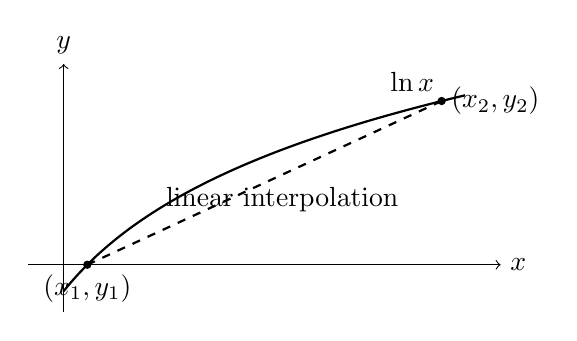
\begin{tikzpicture}[x=1.5cm,y=1.5cm]

        % Axes
        \draw[->] (0.5,0) -- (4.5,0) node[right] {$x$};
        \draw[->] (0.8,-0.4) -- (0.8,1.7) node[above] {$y$};

        % Log function
        \draw[thick,domain=0.8:4.2,samples=100]
            plot (\x,{ln(\x)});

        % Endpoints
        \fill (1,0) circle (1.5pt) node[below] {$(x_1,y_1)$};
        \fill (4,{ln(4)}) circle (1.5pt) node[right] {$(x_2,y_2)$};

        % Linear interpolant
        \draw[dashed,thick] (1,0) -- (4,{ln(4)});

        % Labels
        \node at (3.75,1.55) {$\ln x$};
        \node at (2.65,0.55) {linear interpolation};

    \end{tikzpicture}
    \caption{Linear interpolation of the concave function $\ln x$.
    The interpolating line lies below the function between the two known points.}
\end{figure}


% ------------------------------------------------------------
\subsubsection{ReLU: Rectified Linear Unit}
% ------------------------------------------------------------

A rectified linear unit, or ReLU, is a simple piecewise-linear function defined by

\[
    \boxed{\operatorname{ReLU}(x)=\max(0,x).}
\]

Equivalently,

\[
    \operatorname{ReLU}(x) =
    \begin{cases}
        0, & x<0, \\
        x, & x\geq0.
    \end{cases}
\]

The function is therefore flat for negative inputs and linear for positive inputs.

ReLU functions are widely used as activation functions in neural networks.
Although a single ReLU is extremely simple, combinations of many ReLU units can produce complicated piecewise-linear functions.
Thus ReLUs provide another way of building a complicated function from simple components.


% ------------------------------------------------------------
\subsubsection{Least squares}
% ------------------------------------------------------------

Least squares is a method for finding a model that best represents a collection of data.

Suppose we have measurements

\[
    (x_1,y_1), (x_2,y_2), \ldots, (x_N,y_N)
\]

and a model that predicts values

\[
    \hat{y}_i=f(x_i).
\]

The residual for measurement $i$ is the difference between the observed and predicted values,

\[
    r_i = y_i-\hat{y}_i.
\]

Least squares chooses the parameters of the model so that the sum of the squared residuals is as small as possible,

\[
    \boxed{\text{minimize} \qquad \sum_{i=1}^{N}\left(y_i-\hat{y}_i\right)^2.}
\]

Squaring the residuals prevents positive and negative errors from simply cancelling one another.
The result is the model that gives the smallest total squared discrepancy from the data according to this criterion.
% 
% 
\medskip
\\
\textbf{Legendre's Method}
Adrien-Marie Legendre published the method of least squares in 1805.
He introduced it as a practical method for extracting parameters from astronomical observations when there were more measurements than unknown quantities.
% 
% 
\medskip
\\
\textbf{Gauss' Method}
Carl Friedrich Gauss published his treatment of least squares in 1809.
Gauss claimed that he had been using the method earlier, leading to a historical priority dispute between Gauss and Legendre.
The method became fundamental for fitting mathematical models to noisy experimental observations.


% \paragraph{Common idea}
\bigskip

These methods provide different ways of replacing something complicated by something simpler.
A Taylor expansion represents a function locally using a polynomial.
Linear interpolation represents the function between two known points using a straight line.
ReLU functions provide simple piecewise-linear building blocks from which more complicated functions can be constructed.
Least squares chooses the representation that best matches a collection of measurements according to a specified error measure.


% ============================================================
\subsection{Null hypotheses and probability distributions}
% ============================================================

A useful null hypothesis is the simplest random process that could plausibly generate the observations.
The purpose of the null hypothesis is to ask what behavior we should expect even without invoking an additional mechanism.
Probability distributions provide mathematical descriptions of the fluctuations expected under different random processes.

% ------------------------------------------------------------
\subsubsection{Example: the Buri experiment}
% ------------------------------------------------------------

Peter Buri's experiment provides a classic demonstration of genetic drift in small populations.
Buri studied many independent populations of \textit{Drosophila melanogaster}.
In one experimental series, 107 replicate populations were followed for 19 generations.
Each population was initiated with 16 heterozygous flies.
At every subsequent generation, 8 males and 8 females were randomly selected from the offspring to found the next generation.
The population size was therefore kept small, while the particular alleles passed to the next generation were determined partly by random sampling.
% 
\medskip
\\
\textbf{Allele frequency}
\\
Using the red, orange, and white notation from the lecture, suppose that red flies carry two copies of the red allele, orange flies are heterozygous, and white flies carry no copies of the red allele.
If there are $N_{\mathrm{red}}$ red flies, $N_{\mathrm{orange}}$ orange flies, and $N_{\mathrm{flies}}$ flies in total, then the frequency of the red allele is
\[
    p_{\mathrm{red}} = \frac{2N_{\mathrm{red}}+N_{\mathrm{orange}}}{2N_{\mathrm{flies}}}.
\]

The factor of two in the denominator appears because each diploid fly carries two copies of the locus.
Initially, all 16 flies are heterozygous, so
\[
    p_{\mathrm{red}} = \frac{16}{32} = \frac{1}{2}.
\]

As an example, suppose a later generation contains 4 red, 2 white, and 10 orange flies.
Then
\[
    p_{\mathrm{red}} = \frac{2(4)+10}{2(16)} = \frac{18}{32} = 0.5625.
\]
% 
\medskip
\\
\textbf{Genetic drift}
\\
Even when the two alleles have the same fitness, random sampling means that their frequencies do not remain exactly constant from one generation to the next.
One population may contain slightly more copies of the red allele, while another may contain slightly fewer.
These small fluctuations accumulate over generations.
Different replicate populations therefore wander away from the common initial allele frequency,
\[
    p_{\mathrm{red}}=\frac{1}{2}.
\]
Eventually, some populations reach
\[
    p_{\mathrm{red}}=1,
\]
meaning that the red allele has become fixed.
Others reach
\[
    p_{\mathrm{red}}=0,
\]
meaning that the red allele has been lost and the alternative allele has become fixed.
These states are absorbing: once an allele has disappeared from a closed population, random sampling alone cannot bring it back.
Thus substantial differences between populations can arise from random sampling alone, without invoking a selective advantage.
This random change in allele frequency is called \emph{genetic drift}.

% ============================================================
\subsubsection{Common probability distributions}
% ============================================================

Different stochastic processes naturally give rise to different probability distributions.
Some recurring distributions in physical biology are:
\begin{enumerate}
    \item binomial
    \item Poisson
    \item Gaussian
    \item exponential
    \item geometric
\end{enumerate}

The binomial, Poisson, and Gaussian distributions have already appeared in the course.
The exponential distribution describes an important new class of problems: waiting times.

% ------------------------------------------------------------
\subsubsection{Exponential distribution}
% ------------------------------------------------------------

The exponential distribution describes the waiting time until an event occurs when that event happens with a constant rate.
Let the event occur at rate $\lambda$.
The probability density for the waiting time $t$ is
\[
    \boxed{p(t)=\lambda e^{-\lambda t}, \qquad t\geq0.}
\]
The mean waiting time is
\[
    \langle t\rangle = \frac{1}{\lambda},
\]
and the variance is
\[
    \operatorname{Var}(t)=\frac{1}{\lambda^2}.
\]

% ------------------------------------------------------------
\paragraph{Example: molecular binding times}
% ------------------------------------------------------------

Consider an experiment in which a DNA molecule is immobilized on a slide.
The DNA is fluorescently labeled so that its position can be identified.
A fluorescently labeled DNA-binding protein is then added.
When the protein is bound to the DNA, both the DNA signal and the protein signal are observed at the same location.
The fluorescence signal can therefore be converted into a simple time trace,
\[
    I(t) =
    \begin{cases}
        1, & \text{protein bound}, \\
        0, & \text{protein unbound}.
    \end{cases}
\]
A sequence of binding and unbinding events then appears as alternating intervals in which $I(t)=1$ and $I(t)=0$.
% 
\medskip
\\
\textbf{Bound-state lifetime}
\\
Suppose a bound protein dissociates with a constant rate $k_{\mathrm{off}}$.
Let $S(t)$ be the probability that a protein which was bound at time $t=0$ is still bound after time $t$.
During a small interval $\Delta t$, the probability of dissociation is
% 
\[
    k_{\mathrm{off}}\Delta t.
\]
% 
The probability of remaining bound is therefore
% 
\[
    1-k_{\mathrm{off}}\Delta t.
\]
% 
The update rule is
% 
\[
    S(t+\Delta t)=S(t)\left(1-k_{\mathrm{off}}\Delta t\right).
\]
% 
Taking the continuous-time limit gives
% 
\[
    \frac{\dd S}{\dd t}=-k_{\mathrm{off}}S.
\]
% 
With the initial condition $S(0)=1$,
% 
\[
    \boxed{S(t)=e^{-k_{\mathrm{off}}t}.}
\]
% 
This is the probability that the protein remains bound for at least time $t$.
The probability density for the actual bound lifetime $t_{\mathrm{on}}$ is obtained from
% 
\[
    p(t_{\mathrm{on}})=-\frac{\dd S}{\dd t_{\mathrm{on}}}.
\]
% 
Therefore,
% 
\[
    \boxed{
        p(t_{\mathrm{on}})=k_{\mathrm{off}}e^{-k_{\mathrm{off}}t_{\mathrm{on}}}.
        }
\]
% 
The mean bound lifetime is
% 
\[
    \langle t_{\mathrm{on}}\rangle = \frac{1}{k_{\mathrm{off}}}.
\]
% 
Thus measuring the distribution of bound-state durations provides a way to estimate the dissociation rate $k_{\mathrm{off}}$.
% 
\medskip
\\
\textbf{Waiting for binding}
\\
The unbound intervals can be treated similarly.
If binding occurs with an effective constant rate $\lambda_{\mathrm{on}}$, then
% 
\[
    p(t_{\mathrm{off}})=\lambda_{\mathrm{on}}e^{-\lambda_{\mathrm{on}}t_{\mathrm{off}}}.
\]
% 
If $k_{\mathrm{on}}$ is a bimolecular association rate constant and the protein concentration is $[P]$, then the effective rate is
% 
\[
    \lambda_{\mathrm{on}}=k_{\mathrm{on}}[P].
\]
% 
The important distinction is therefore
% 
\[
    \text{bound lifetime} \longleftrightarrow k_{\mathrm{off}},
\]
% 
whereas
% 
\[
    \text{unbound waiting time} \longleftrightarrow k_{\mathrm{on}}[P].
\]

% ------------------------------------------------------------
\subsubsection{Summary of probability distributions}
% ------------------------------------------------------------

See table~\ref{tab: prob_distributions}.

\begin{table}[h!]
\centering
\small
\renewcommand{\arraystretch}{1.6}

\begin{tabularx}{\textwidth}{
    |>{\raggedright\arraybackslash}p{2.5cm}
    |>{\raggedright\arraybackslash}p{5.5cm}
    |>{\centering\arraybackslash}p{1cm}
    |>{\centering\arraybackslash}p{1.6cm}
    |>{\raggedright\arraybackslash}X|
}
\hline
\textbf{Distribution} &
\textbf{PMF/PDF} &
\textbf{Mean} &
\textbf{Variance} &
\textbf{Representative examples}
\\
\hline
Binomial \newline \newline \miniBinomial & 
$\displaystyle P(k)=\binom{n}{k}p^k(1-p)^{n-k}$ &
$np$ &
$np(1-p)$ &
Receptor occupancy among $n$ independent receptors; rightward steps in an $n$-step random walk; protein partitioning at cell division.
\\
\hline
Poisson \newline \newline \miniPoisson & 
$\displaystyle P(k)=e^{-\lambda}\frac{\lambda^k}{k!}$ &
$\lambda$ &
$\lambda$ &
Mutations per genome; deaths from horse kicks per army corps; wartime bomb hits per district; photons detected during a fixed time interval.
\\
\hline
Gaussian \newline \newline \miniGaussian & 
$\displaystyle p(x)=\frac{1}{\sqrt{2\pi\sigma^2}}\exp\left[-\frac{(x-\mu)^2}{2\sigma^2}\right]$ &
$\mu$ &
$\sigma^2$ &
Errors in repeated measurements; displacement after many diffusive steps; polymer end-to-end displacement; variation in human height.
\\
\hline
Exponential \newline \newline \miniExponential &
$\displaystyle p(t)=\lambda e^{-\lambda t}$ &
$\displaystyle \frac{1}{\lambda}$ &
$\displaystyle \frac{1}{\lambda^2}$ &
Waiting time until radioactive decay; time between constant-rate events; lifetime of a molecular state; waiting time until the next photon.
\\
\hline
Geometric \newline \newline \miniGeometric &
$\displaystyle P(n)=(1-p)^n p$ &
$\displaystyle \frac{1-p}{p}$ &
$\displaystyle \frac{1-p}{p^2}$ &
Failures before the first success; unsuccessful chromosome-capture attempts; tails before the first head; rejected proofreading attempts.
\\
\hline
\end{tabularx}

\caption{Common probability distributions and representative examples.
The geometric distribution is defined here as the number of failures before the first success.}
\label{tab: prob_distributions}
\end{table}




The distributions describe different kinds of random variables and different underlying stochastic processes.
The binomial distribution describes the number of successes in a fixed number of independent trials.
The Poisson distribution describes the number of events occurring when independent events happen at a constant average rate.
The Gaussian distribution commonly arises when a quantity is the sum of many independent contributions.
The exponential distribution describes the waiting time until the next event in a constant-rate process.
The geometric distribution is the discrete analogue of the exponential distribution and describes how many independent trials occur before the first success.

